\documentclass[tikz, border=4mm]{standalone} 
\usetikzlibrary{positioning, fit, calc}
\tikzset{block/.style={draw, thick, text width=2cm, minimum height=1.2cm, align=center},
add/.style={draw,thick,circle,minimum height=0.5cm,},
line/.style={-latex,thick}
}
\begin{document}

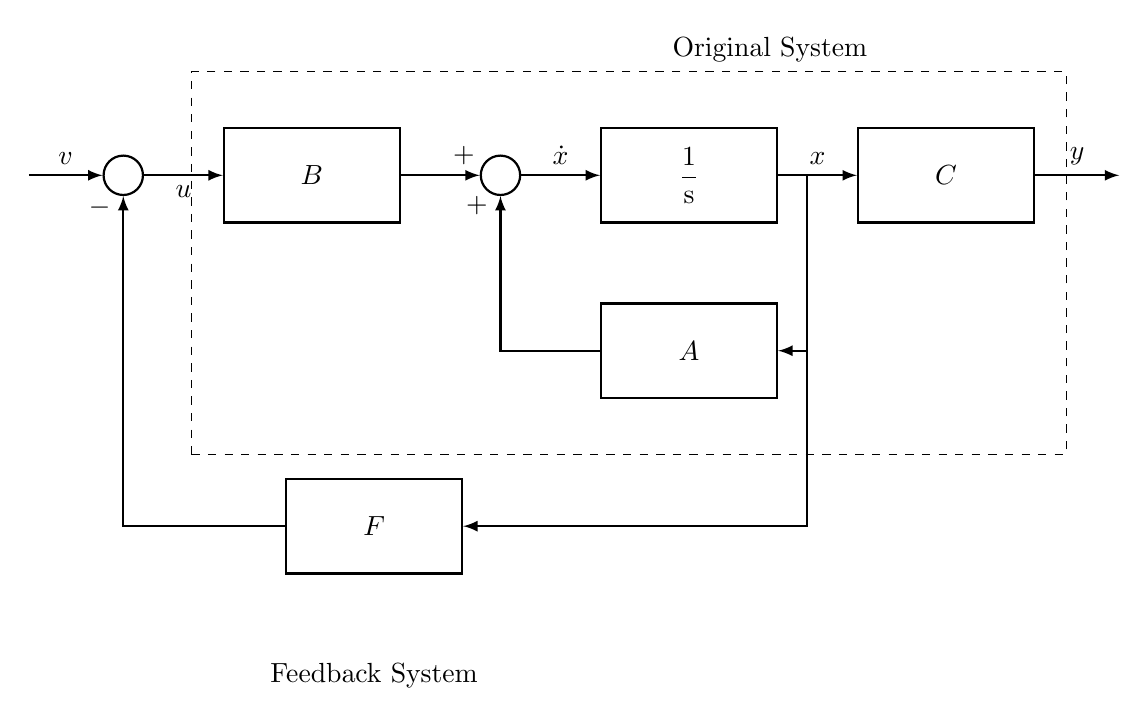
\begin{tikzpicture}
    \node[add](FeedAdd){};
    \node[block,right=of FeedAdd](B){$B$};

    \node[add,right=of B](OrgAdd){};
    \node[block,right=of OrgAdd](init){$\displaystyle \frac{1}{\rm{\bm s}}$};
    \node[block,right=of init](C){$C$};

    \node[block,below=of init](A){$A$};
    \node[block,below=of A,xshift=-4cm](F){$F$};

    \node[draw,dashed, inner xsep=4mm, inner ysep=7mm, fit=(B)(C)(A), label={80:Original System}]{};
    \node[below=of F]{Feedback System};

    \draw[line] (FeedAdd)+(-1.2cm,0) -- node[above]{$v$}(FeedAdd);
    \draw[line] (FeedAdd) -- node[below]{$u$}(B);
    \draw[line] (B) -- node[above,xshift=0.3cm]{$+$}(OrgAdd);
    \draw[line] (OrgAdd) -- node[above]{$\dot{x} $}(init);
    \draw[line] (init) -- node[above]{$x$}(C);
    \draw[line] (C) -- node[above]{$y$}+(2.2cm,0);

    \draw[line] (init) -- ++(1.5cm,0) |- (A);
    \draw[line] (init) -- ++(1.5cm,0) |- (F);
    
    \draw[line] (A) -| node[above,xshift=-0.3cm,yshift=1.6cm]{$+$}(OrgAdd);

    \draw[line] (F) -| node[above,xshift=-0.3cm,yshift=3.8cm]{$-$}(FeedAdd);

\end{tikzpicture}
\end{document}